\chapter{Robotics middleware}



\section{Introduction}

Robotic systems require complex infrastructure to be able to operate correctly. With numerous different parts working together that have to communicate and coordinate, these systems need a robust way to enable such communication. At the same time, translating user commands into instructions that can be understood by the inner electronics of the robot is a complex process that should only be exposed to qualified operators.

Robotics middleware is a type of software that provides utilities to software applications used in complex robot control systems. It is sometimes referred to as "software glue" because it links together different software components to create a complete system. Using a robotics middleware is a solution to the problems defined above: the middleware facilitates communication, provides a way to package software in a structured manner, and enables hardware abstractions to make development easier.

In this chapter, we introduce ALFRED as a robotics middleware. It follows the structure of UNIX-like operating systems, with separation of privileges between system programmers and normal users. It enables communication between software components with an external message passing system. It allows robotics application designers to create interactions with robotic arms without the need for specialized education or to learn the inner workings of a robotic arm. Finally, it provides access to software utilities and a hardware abstraction layer to simplify the surrounding parts of developing robotics applications.



\section{Related work}

ROS \cite{ros} was explored to use as a robotics middleware. ROS is a set of software pieces to help the development of robotics applications. It provides hardware abstraction, low-level device control, implementation of commonly used functionality, message-passing between processes, and package management. It enables two-way communication via topics. Components can subscribe to topics to receive messages, but also publish to topics to send messages. Software comes in the form of packages, which are units that can be run, used as dependencies or for configuration.

Another middleware is ISAAC, a solution by NVIDIA specialized for, but not limited to, high compute situations. ISAAC links together software in a graph structure, where nodes are the computational software pieces and edges are the exchange of data between the nodes. Custom applications can be created to implement functionality to robotics systems and be integrated into ISAAC as nodes. ISAAC also gives access to tools for simulation and training of deep learning models. With ISAAC GEMs, users can add AI-enabled data processing with pre-trained models.



\section{Architecture overview}

ALFRED is built around a publish/subscribe model database that enables inter-component communication. The middleware follows the structure of UNIX-like operating systems, with a Kernel and a Userspace. Robotics applications developed by the users run in the Userspace, while critical components run in the Kernel. The Kernel and Userspace are separated by the \Gls{pubsub} messaging system, which creates a clear border between the two layers of the middleware. We use this clear border to manage the software's permissions over the hardware: we disable hardware access to the Userspace and only make the hardware accessible by the Kernel. To access data from the hardware, the Userspace has to go through the Kernel first, by using the \Gls{pubsub}. Our middleware's architecture is demonstrated in figure \ref{fig:arch_simple}.

\begin{figure}
  \centering
  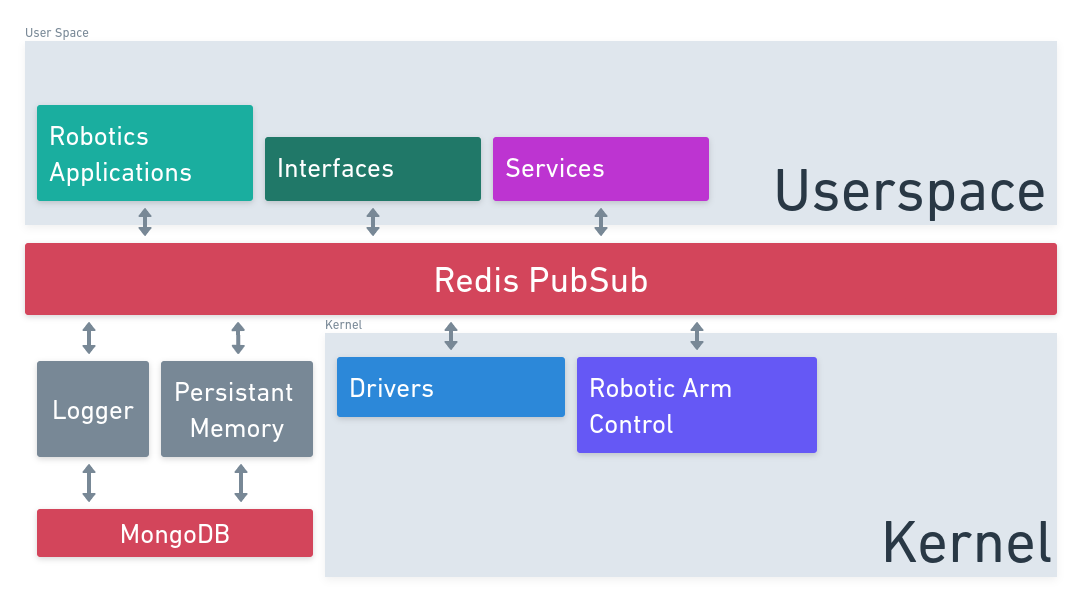
\includegraphics{images/ALFRED_arch_simple.png}
  \caption{ALFRED's architecture}
  \label{fig:arch_simple}
\end{figure}

The middleware runs in Docker \cite{docker} and is deployed with Docker Compose \cite{docker-compose}. Each component is deployed as a separate container. Using containers to deploy our software makes it easier to separate the different parts of the system but also handle dependencies. Networks\sidenote{Networks are part of Docker and enable containers to communicate with each other whereas they would normally be isolated.} are used to enable communication between components selectively. We use environment variables to configure global behavior at runtime, e.g. if the real arm should move or not.

\paragraph{Kernel}

The Kernel is the core of the middleware. It has complete control over the robot arm. It contains a Hardware Abstraction Layer (which we call the drivers) and the robotic arm control software. Drivers are the interface between external devices, such as cameras, and the Kernel. They can get data from and send commands to the devices. On the other hand, the Robotic arm control component contains the \gls{api} for moving the robotic arm, as well as utilities to manage its state (starting, stopping, handling disconnections\dots).

\paragraph{Userspace}

Userspace contains user-created components. To house user-created software, we developed the Robotics Applications Component (RAC), the interfaces and the services. The RAC contains applications, which are pieces of software that interact with the arm and implement the functionalities. Applications are modular: they can be developed outside of our middleware and integrated later with minimal changes thanks to a plug-and-play structure. Interfaces are ways to visualize what is happening in the system and interact with it in a user-friendly way. Services are components that are used to compute data but do not interact with the arm, like deep learning algorithms. They can also be used by multiple applications.

\paragraph{Inter-component communication}

Components communicate with each other using a \gls{pubsub} messaging system. This component sits between Kernel and Userspace and prevents them from interacting directly with each other. Instead, all communication has to go through the \gls{pubsub}. It provides a clear separation between Kernel and Userspace, and is our implementation of \glspl{os_ring}, or hardware access restriction. The Kernel is at ring 0 (no restrictions, most privileged) and Userspace at ring 1 (more restrictions, less privileged).




\section{Kernel}


\subsection{Related work}

\subsubsection{Robotic arm control}

Most robotic arms have an API exposing functions that allow users to control the arm more easily. Instead of controlling each of the arm's motors individually, the API exposes functions to execute complex movements, such as moving the arm to a certain position in space in a straight line, or drawing a curve from one point to the other with a certain radius.

Internally, the robotic arm's controller still translates user commands into individual motor movements. Most robotic arms provide a way for experienced developers to send these individual motor movements directly to the arm, thus reducing the load on the onboard controller. These movements can be obtained manually via mathematics, but software like PyBullet\cite{pybullet} or MATLAB\cite{MATLAB} makes it easier. They provide utilities to specify robot-specific parameters, like the number of degrees of freedom and the length of the links between the motors, from existing data. Without these tools, the programmer would have to compute these parameters themselves. They can also provide access to simulation, creating a digital copy of the robotic arm to predict behavior ahead of time.

\subsubsection{Drivers}

In the Linux kernel, drivers are implemented as modules which can be added or removed. They are written in C or Assembly for low level control over the hardware, and they expose a file which presents the data from the hardware once it has been acquired and treated. Each driver exposes a set of functions which can be called to generate data or interact with the device.

In ROS, drivers are implemented as packages, like any other software piece, that produce data to a topic. These drivers are one or more layers above the raw hardware drivers of the Linux kernel. They often use libraries which read from the device files and expose this data in a more readable format. ROS drivers are flexible in that they don't need to stream all the data all the time; instead, they can be made to output data only when something significant happens, like when a spike of current is detected from a sensor, so they can arbitrarily abstract the data for the target software.


\subsection{Robotic arm control}

The Robotic arm control component is implemented in Python 3.9 and is deployed as a container. The component is tasked with receiving commands and data from the whole system and moving the robotic arm. Its algorithm is described in \ref{alg:controller}.

\begin{algorithm}
  \caption{Robotic arm control}
  \label{alg:controller}
  \While{true}{
    $message\leftarrow$ message from pub/sub\;
    \If{$message$ is not empty}{
      parse $message$\;
      \If{$message$ is a command}{
        execute $message$ on robot arm\;
      }
      \ElseIf{$message$ is data}{
        save and use $message$\;
      }
    }
  }
\end{algorithm}


\subsection{Drivers}

Drivers are implemented in Python 3.9 and are deployed as a container. The container has full access to the host machine's hardware to be able to read and manipulate external devices. In the container, each driver is started as a background process, allowing it to run concurrently with the other drivers. When every driver is started, the parent process runs an infinite loop to keep the drivers running. Drivers have two main components: the \lstinline{DataProducer} and the \lstinline{CommandGetter}, which are started as threads and run indefinitely. They communicate with the rest of the system via the \gls{pubsub}. Topics used by the drivers have a special nomenclature, which is \lstinline{device-data-<device name>} for the \lstinline{DataProducer} and \lstinline{device-command-<device name>} for the \lstinline{CommandGetter}. Here are the algorithms for the \lstinline{CommandGetter} \ref{alg:command_getter} and the \lstinline{DataProducer} \ref{alg:data_producer}:

\begin{algorithm}
  \caption{CommandGetter}
  \label{alg:command_getter}
  \KwData{$topic\leftarrow$ "device-command-<device name>"}
  \While{true}{
    $command\leftarrow$ command from pubsub\;
    \If{$command$ is not empty}{
      parse $command$\;
      send $command$ to device\;
    }
  }
\end{algorithm}

\begin{algorithm}
  \caption{DataProducer}
  \label{alg:data_producer}
  $topic\leftarrow$ "device-data-<device name>"\;
  \While{true}{
    $data\leftarrow$ data from device\;
    \If{$data$ is not empty}{
      publish $data$ to $topic$\;
    }
  }
\end{algorithm}

Currently, drivers are implemented for these devices:
\begin{itemize}
  \item Realsense D435 cameras
  \item BLTouch sensors with a microcontroller as an intermediary data via Serial communication
  \item Microphones
\end{itemize}

The behavior of the drivers can be customized by environment variables set in the Docker Compose file.



\section{Userspace}


\subsection{Related work}

\subsubsection{Robotics applications}

In ROS, applications can be launched via the command line, but also programmatically using the roslaunch API. This requires to create a launch file specifying parameters for the application.

Outside of ROS, programs often expose APIs to make interaction possible. These API use protocols to structure communication, mainly REST (Representational State Transfer) and RPC (Remote Procedure Call). RPC is suited to executing applications from outside but has limited compatibility with the web. Thus, we considered three REST API frameworks from Python:

\begin{itemize}
  \item Flask
  \item Django
  \item FastAPI
\end{itemize}

Flask is a minimal web framework which contains basic features such as routing, debug and static files.

Django is a more heavyweight framework for creating complex websites with an SQL database as its centerpoint. It follows the Model-View-Controller pattern and has many features including an auto-generated admin panel.

FastAPI is a web framework built on top of Starlette, an ASGI (Asynchronous Server Gateway Interface) framework/toolkit. FastAPI has all the features of Flask with added functionality, such as OpenAPI docs generation and async support.


\subsection{Robotics applications}

The robotics applications component (RAC) is implemented in Python 3.9 and is deployed as a container. The RAC gives access to the robotic arm control component to the user. The RAC and the robotic arm control component communicate with each other via the \Gls{pubsub}. The API uses FastAPI \cite{fastapi} as its main technology. The RAC contains the applications which implement functionality on the robot arm. Applications can be called or interacted with via HTTP requests. To manage applications within the software, we created a class called \lstinline{Apps} class, which is a subclass of Python's \lstinline{multiprocessing.Process}. The \lstinline{Apps} class provides utilities to start applications, check if they are running, handle exceptions and provide two way communication between the application and the RAC.

Applications are managed by the RAC's \lstinline{ContextManager}, which is tasked with starting and stopping apps. The \lstinline{ContextManager} only allows for one application to run at a time, to avoid conflicts if two applications wanted to move the robotic arm at the same time.

Applications are separate processes with their own separate memory, instead of threads that share their memory with their parent. This helps avoid errors with memory management, and bypasses the restrictions of some libraries used, e.g. OpenCV not being able to show windows in anything other than the main thread.

Applications can be developed outside of our middleware and later integrated thanks to the structure of the RAC \ref{fig:api_file_structure}: applications are kept separate from the rest of the API, and live side by side. To expose an application, a route\sidenote{HTTP method (\lstinline{GET}, \lstinline{POST}, ...), path (ex: \lstinline{/applications/grasping}), and handler combination.} needs to be created. The route is then added to the applications router\sidenote{Part of the software that determines which route receives a specific request.} which is itself added to the main router.

\begin{figure}[h]
  \centering
  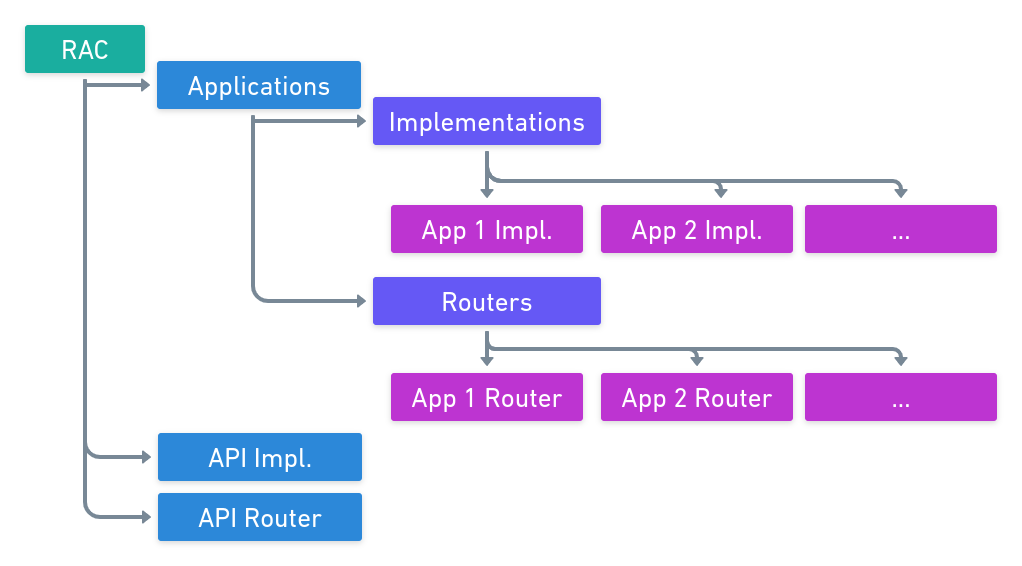
\includegraphics{images/API_file_structure.png}
  \caption{File structure of the RAC (simplified)}
  \label{fig:api_file_structure}
\end{figure}


\subsubsection{Evaluation}

Students were tasked with developing applications using ALFRED.
One of them created a driver for a BLTouch bed leveling device interfaced with a micro-controller, and an application using this device to create a 3D map of any mostly flat surface.
Another created an interface plugging into the middleware to act as a dashboard, showing system information and executing applications.
Here were their remarks about the system:

\begin{itemize}
  \item The application was able to be developed outside of the middleware and then integrated with minimal changes, in less than a day.
  \item Creating the application didn't require extensive knowledge about robotics or the robot arm.
  \item The driver was conceived with few (about 30 added) lines of code from a basic template.
  \item The data exposed by the RAC allowed the dashboard to show meaningful system data such as the current position of the robot.
  \item The dashboard was able to be developed outside of the system and then integrated only by setting up the appropriate Docker environment.
\end{itemize}


\subsection{Services}

Services are implemented as Docker containers. Since they are a bit more generic, the user is responsible for specifying the dependencies for their services in the component's \lstinline{Dockerfile}. Examples for services are a Natural Language Processing server or an API for external programs such as Unity. We separated services from robotics applications because some services could require different versions of Python, or even a completely different runtime environment. At the moment, services have to be added manually into the whole middleware's Docker Compose file.


\subsection{Human-Robot Interfaces}

Interfaces are a type of service meant to handle input and output from the user. An example of interface is a Web dashboard for viewing the status of the system and managing applications.



\section{Inter-component communication}


\subsection{Related work}

Message handling can be done with ROS via its topics. Messages can be sent by pieces of software to a specific topic, and other pieces of software can subscribe to topics to get the messages. Messages are defined by a \lstinline{type} which defines the structure of the message and allows ROS to automatically parse messages.

Redis is another solution for realtime communication between processes, specifically its \Gls{pubsub} module. Redis Pub/Sub uses channels where publishers can push data and subscriber can subscribe to get data. Messages don't have types which means the publisher is responsible for encoding the data and the subscriber is responsible for decoding it but the communication was found to be faster than ROS \cite{redis_benchmark}.

Other solutions for inter-process communication include D-Bus. D-Bus is based around a message bus daemon which applications connect to. Applications use a library, libdbus, to interact with the message bus. The daemon acts as a router, sending messages from one application to another. Communication is one-to-one only.


\subsection{Communication bus}

Inter-component communication is done with Redis \cite{redis}, specifically Redis' \Gls{pubsub} implementation. It runs in a Docker container from the Bitnami image, \lstinline{bitnami/redis} version 7.0 with default settings. The \Gls{pubsub} sits in-between the Kernel and Userspace and allows components to send each other data.


\subsection{Persistent storage}

The Redis Pub/Sub doesn't persist the data it receives to disk, so MongoDB is used for long-term storage. Data stored includes logs and component-specific data, but it can also serve as a way to save messages sent via the \Gls{pubsub}. The Kernel possesses its own database for storing system-critical data, while the data from the Userspace database can be accessed by both Userspace and Kernel.



\section{Conclusion}


\subsection{Applications}

In this chapter, we described an infrastructure for developing applications on robotic arms. It follows the architecture of UNIX-like operating systems with its separation into Kernel and Userspace and the associated \glspl{os_ring} to define privileges.

This middleware makes developing robotics applications accessible to users with limited knowledge about robotics and robotic arms. It means that developers need less training and that they can have more confidence that their software won't cause damage on the system.

Thanks to its modular architecture, software can be created outside of the system and integrated later with minimal modifications. This is useful since debugging becomes harder the more complex a system is. With isolated software, developers can find and fix issues more rapidly.

With the use of a central \Gls{pubsub} messaging system, components don't need to know who they are sending their data to, but only need to determine the name of a channel that the relevant software can listen on. With this, we can reduce how strongly components depend on each other, which is called coupling. Reduced coupling makes breaking changes less frequent when modifying related code since the components communicating are not directly linked to each other.


\subsection{Limitations}

Running every component as Docker containers adds a complexity that would not exist with native execution. The robotics applications component still has to be run in \lstinline{privileged} mode\sidenote{Privileged: has access to every device. Unprivileged: cannot use the host computer's devices.}, because some applications require access to the screen to show information. Running in \lstinline{privileged} mode diminishes the usefulness of having a separation between Kernel and Userspace, since in the end Userspace can still access devices directly.

Running in Docker also means components are difficult to debug once they have been integrated into the system. This is because every time a modification has to be done, the system needs to be stopped, built, and then started again for the changes to be taken into account. Approximate times are shown in table \ref{table:restart_times_docker}. Build times can be especially long when dependencies are changed and the whole image has to be rebuilt. Setup times can also be long depending on the applications, e.g. when loading a deep learning model. Such long restart times decrease the efficiency at which the project can be iterated on.

\begin{table}[ht]
  \centering
  \caption{System restart times.}
  \label{table:restart_times_docker}
  \begin{tabular}[t]{lcc}
    \hline
                  & Time (best, seconds) & Time (worst, seconds) \\
    \hline
    Stop      & 20           & 30           \\
    Build     & 20           & 600+         \\
    Start     & 20           & 30           \\
    Setup     & 10           & 300+         \\
    \hline
    Total     & 70           & 960+         \\
    \hline
  \end{tabular}
\end{table}%

As it is, the controller is using ALFRED's specific robot arm's API to move the arm.
This means that applications developed for this specific robotic arm will not be compatible on another arm.
It also means that the control of the finite movements of the robotic arm comes from an external program, and so the middleware's controller component can't directly influence said control.


\subsection{Future works}

Issues with the API running in \lstinline{privileged} mode can be solved by delegating the responsibility of showing information to the Kernel. An interface could be implemented to get image buffers from applications in Userspace and then show these image buffers on screen. Options for configuration would need to be added to respond to the needs of applications in terms of interface. Also, since window controls would be under ownership of the Kernel, applications wouldn't be able to capture user input by themselves, so the Kernel would need to pass these inputs through to the applications.

Some methods were used during development to reduce restart times, but they are not properly integrated and impractical to use by the general public. We plan on creating a fully integrated \lstinline{dev} mode for the system. \lstinline{Dev} mode would enable programmers to make changes without having to rebuild the whole system. This mode would add a feature to automatically reload the Docker container's program(s) when a file is changed or upon user request. Files in the host computer would need to be synchronized with the files inside of the containers, which can be done with Docker \lstinline{volumes}.

As they are implemented currently, services and interfaces are not very well integrated into the system. Indeed, the user has to create their Docker image on their own, add it to the main Compose file, and configure it properly. We want to make services and interfaces easier to add to the system by automating the discovery and integration of services into ALFRED. This piece of software would expose utilities to add new entries in the main Compose file securely with a template. It would allow experienced users to provide their own Docker images, program files, and configuration manually, and less experienced users to use common configurations to quickly and easily deploy new services.

We plan on generalizing the middleware for every robotic arm. To do so, we could first create a mapping between our generalized API for robotic movement and the associated function for every robotic arm. This would change the function that is called within robotic arm control depending on the model of the robotic arm used, but wouldn't change the function called in Userspace. Later, we would step away from using the robotic arms' APIs, and compute the robot's movements ourselves using Inverse Kinematics, only sending motor movements to the robotic arms.
